% This must be in the first 5 lines to tell arXiv to use pdfLaTeX, which is strongly recommended.
\pdfoutput=1
% In particular, the hyperref package requires pdfLaTeX in order to break URLs across lines.

\documentclass[11pt]{article}

% Change "review" to "final" to generate the final (sometimes called camera-ready) version.
% Change to "preprint" to generate a non-anonymous version with page numbers.
\usepackage[review]{acl}

% Standard package includes
\usepackage{times}
\usepackage{latexsym}
\usepackage{amsmath}
\usepackage[T1]{fontenc}
\usepackage{tabularx}
\usepackage[utf8]{inputenc}

\usepackage{microtype}

\usepackage{inconsolata}

\usepackage{graphicx}


\title{Instructions for *ACL Proceedings}

% Author information can be set in various styles:
% For several authors from the same institution:
% \author{Author 1 \and ... \and Author n \\
%         Address line \\ ... \\ Address line}
% if the names do not fit well on one line use
%         Author 1 \\ {\bf Author 2} \\ ... \\ {\bf Author n} \\
% For authors from different institutions:
% \author{Author 1 \\ Address line \\  ... \\ Address line
%         \And  ... \And
%         Author n \\ Address line \\ ... \\ Address line}
% To start a separate ``row'' of authors use \AND, as in
% \author{Author 1 \\ Address line \\  ... \\ Address line
%         \AND
%         Author 2 \\ Address line \\ ... \\ Address line \And
%         Author 3 \\ Address line \\ ... \\ Address line}

\author{First Author \\
  Affiliation / Address line 1 \\
  Affiliation / Address line 2 \\
  Affiliation / Address line 3 \\
  \texttt{email@domain} \\\And
  Second Author \\
  Affiliation / Address line 1 \\
  Affiliation / Address line 2 \\
  Affiliation / Address line 3 \\
  \texttt{email@domain} \\}

%\author{
%  \textbf{First Author\textsuperscript{1}},
%  \textbf{Second Author\textsuperscript{1,2}},
%  \textbf{Third T. Author\textsuperscript{1}},
%  \textbf{Fourth Author\textsuperscript{1}},
%\\
%  \textbf{Fifth Author\textsuperscript{1,2}},
%  \textbf{Sixth Author\textsuperscript{1}},
%  \textbf{Seventh Author\textsuperscript{1}},
%  \textbf{Eighth Author \textsuperscript{1,2,3,4}},
%\\
%  \textbf{Ninth Author\textsuperscript{1}},
%  \textbf{Tenth Author\textsuperscript{1}},
%  \textbf{Eleventh E. Author\textsuperscript{1,2,3,4,5}},
%  \textbf{Twelfth Author\textsuperscript{1}},
%\\
%  \textbf{Thirteenth Author\textsuperscript{3}},
%  \textbf{Fourteenth F. Author\textsuperscript{2,4}},
%  \textbf{Fifteenth Author\textsuperscript{1}},
%  \textbf{Sixteenth Author\textsuperscript{1}},
%\\
%  \textbf{Seventeenth S. Author\textsuperscript{4,5}},
%  \textbf{Eighteenth Author\textsuperscript{3,4}},
%  \textbf{Nineteenth N. Author\textsuperscript{2,5}},
%  \textbf{Twentieth Author\textsuperscript{1}}
%\\
%\\
%  \textsuperscript{1}Affiliation 1,
%  \textsuperscript{2}Affiliation 2,
%  \textsuperscript{3}Affiliation 3,
%  \textsuperscript{4}Affiliation 4,
%  \textsuperscript{5}Affiliation 5
%\\
%  \small{
%    \textbf{Correspondence:} \href{mailto:email@domain}{email@domain}
%  }
%}
% !TEX root = paper-main.tex
% Logic for inline comments
\newif\ifshowcomments
% Switch to \showcommentsfalse to turn off comments!
% \showcommentsfalse
\newcommand\todo{\textcolor{red}}
\newcommand{\st}[1]{{\textcolor{teal}{ST:#1}}}
\newcommand{\cd}[1]{\textcolor{blue}{CD:#1}}


%%editing macros
\newcommand{\cut}[1]{}
\newcommand{\xhdr}[1]{\paragraph{#1.}}

%% Terminology macros
\newcommand{\forecastingmodel}{conversational forecasting model\xspace}


\begin{document}
\maketitle
\begin{abstract}
This document is a supplement to the general instructions for *ACL authors. It contains instructions for using the \LaTeX{} style files for ACL conferences.
The document itself conforms to its own specifications, and is therefore an example of what your manuscript should look like.
These instructions should be used both for papers submitted for review and for final versions of accepted papers.
\end{abstract}

\section{Introduction}
The setting of online conversations has become ubiquitous and commonplace. 
Although this has provided new opportunities for civil discourse, online conversations have also become increasingly associated with negative conversational phenomenon such as toxicity, hate speech, and personal attacks~\citep{Cheng_Danescu-Niculescu-Mizil_Leskovec_2021}.
In particular, seemingly calm beginnings to online discussions can devolve into heated personal attacks. 
Prior work has termed this phenomenon as conversations gone awry (CGA)~\citep{zhang-etal-2018-conversations, chang-danescu-niculescu-mizil-2019-trouble}.

Predicting when conversations will go awry is a natural task to try and automate. 
Building a model that can effectively predict this phenomenon would be useful in online discussion forums such as Reddit or Wikipedia talk pages. 
If the model flags a conversation as potentially derailing, then moderators could step in and prevent users from further escalating the conversation. 
This would help make these online discussion forums a more friendly and welcoming space. 

Recent studies have focused on developing models for the task of forecasting when conversations will go awry~\citep{zhang-etal-2018-conversations, chang-danescu-niculescu-mizil-2019-trouble, Yuan_Singh_2023}. 
These models use a combination of linguistic markers (e.g., politeness) and unsupervised learning to make early predictions. 
The difficulty of this task lies in the early prediction aspect - the model is unable to see the actual personal attack before making its prediction. 
State-of-the-art (SOTA) models are only able to achieve an accuracy of slightly less than 70\% on CGA benchmarks~\citep{zhang-etal-2018-conversations, chang-danescu-niculescu-mizil-2019-trouble, Yuan_Singh_2023}. 

This performance leaves much to be desired. 
The prior work that developed the models does not carefully examine how the model makes its predictions. 
Further understanding of the model and its shortcomings would pave the way for future improvements on the CGA task. 
In particular, this project investigated the model's use of the conversational context in making its predictions. 

We wanted to understand two main research questions.
\begin{enumerate}
    \item Is understanding the conversational context essential for SOTA model performance?
    \item Do SOTA models utilize the conversational context when making forecasts?
\end{enumerate}
We hypothesized that conversational context was not actually necessary for the model's performance, and that the model was not utilizing the context when making forecasts. 

This project answers these questions by modifying and creating new contexts for the model to make forecasts with. 
We could then see how the model's predictions changed as a result of the new context. 
Ultimately, we found that SOTA models do not need conversational context for their performance, but that they do in fact utilize conversational contexts when making their forecasts. 
These results suggest that the current CGA benchmark may not be difficult enough, and that a new benchmark is needed to help train and improve model performance. 

\section{Engines}

To produce a PDF file, pdf\LaTeX{} is strongly recommended (over original \LaTeX{} plus dvips+ps2pdf or dvipdf). Xe\LaTeX{} also produces PDF files, and is especially suitable for text in non-Latin scripts.
\section{Task Formulation}
In a simple scenario, the CGA forecasting task can be formulated as a classification problem, mathematically expressed as:
\begin{equation}
p_{\mathrm{derailment}} = f(\mathrm{context})
\label{eq:classification}
\end{equation}
where $f$ is a classification model, \emph{context} represents a static snapshot of the conversation at a specific point in time, and $p_{\mathrm{derailment}}$ is the predicted probability of derailment as output by $f$.

In real-world applications, however, derailment forecasting must occur dynamically, following each utterance in an ongoing conversation. This introduces additional complexities, requiring a temporal dimension to Equation \ref{eq:classification}:
\begin{equation}
p_{\mathrm{event}}(t) = f(\mathrm{context}(t))
\label{eq:forecastingmodel}
\end{equation}

In this formulation, the CGA model produces \emph{multiple} utterance-level forecasts throughout the lifetime of a conversation. However, each conversation is associated with a single ground-truth label, making it unsuitable to treat each forecast as an independent prediction. This necessitates adjustments to both the prediction process and the evaluation methodology.

Under the static classification framework (Equation \ref{eq:classification}), a single prediction corresponds to a specific timestamp in the conversation, referred to as the \textbf{utterance-level} prediction. In contrast, dynamic forecasting requires \emph{aggregating} multiple utterance-level predictions over the course of a conversation to generate a single prediction that can be compared with the ground-truth label.

In this work, we adopt an evaluation approach informed by previous research. Specifically, a conversation is forecasted to derail if any utterance-level prediction exceeds a threshold determined on the development set. This thresholding mechanism aggregates predictions across utterances, producing the final \textbf{conversation-level} forecast. The highest utterance-level forecast for a conversation is used as the conversation-level prediction for evaluation purposes.
\section{Data}

This project uses the CGA datasets.
This consists of two separate datasets: Reddit ChangeMyView (CMV) and Wikipedia talk pages~\citep{chang-danescu-niculescu-mizil-2019-trouble,zhang-etal-2018-conversations}.
The CGA-CMV dataset consists of $20,576$ conversations from the CMV subreddit.
A conversation is considered to go awry if it eventually has a comment removed by a moderator for violating Rule 2 of the subreddit: "Don't be rude or hostile to other users."
The CGA-Wiki dataset consists of $4,188$ conversations from Wikipedia talk pages.
The conversations were labeled by crowdworkers as either containing a personal attack or staying calm throughout.

\section{Document Body}

\subsection{Footnotes}

Footnotes are inserted with the \verb|\footnote| command.\footnote{This is a footnote.}

\subsection{Tables and figures}

See Table~\ref{tab:accents} for an example of a table and its caption.
\textbf{Do not override the default caption sizes.}

\begin{table}
  \centering
  \begin{tabular}{lc}
    \hline
    \textbf{Command} & \textbf{Output} \\
    \hline
    \verb|{\"a}|     & {\"a}           \\
    \verb|{\^e}|     & {\^e}           \\
    \verb|{\`i}|     & {\`i}           \\
    \verb|{\.I}|     & {\.I}           \\
    \verb|{\o}|      & {\o}            \\
    \verb|{\'u}|     & {\'u}           \\
    \verb|{\aa}|     & {\aa}           \\\hline
  \end{tabular}
  \begin{tabular}{lc}
    \hline
    \textbf{Command} & \textbf{Output} \\
    \hline
    \verb|{\c c}|    & {\c c}          \\
    \verb|{\u g}|    & {\u g}          \\
    \verb|{\l}|      & {\l}            \\
    \verb|{\~n}|     & {\~n}           \\
    \verb|{\H o}|    & {\H o}          \\
    \verb|{\v r}|    & {\v r}          \\
    \verb|{\ss}|     & {\ss}           \\
    \hline
  \end{tabular}
  \caption{Example commands for accented characters, to be used in, \emph{e.g.}, Bib\TeX{} entries.}
  \label{tab:accents}
\end{table}

As much as possible, fonts in figures should conform
to the document fonts. See Figure~\ref{fig:experiments} for an example of a figure and its caption.

Using the \verb|graphicx| package graphics files can be included within figure
environment at an appropriate point within the text.
The \verb|graphicx| package supports various optional arguments to control the
appearance of the figure.
You must include it explicitly in the \LaTeX{} preamble (after the
\verb|\documentclass| declaration and before \verb|\begin{document}|) using
\verb|\usepackage{graphicx}|.

\begin{figure}[t]
  \includegraphics[width=\columnwidth]{example-image-golden}
  \caption{A figure with a caption that runs for more than one line.
    Example image is usually available through the \texttt{mwe} package
    without even mentioning it in the preamble.}
  \label{fig:experiments}
\end{figure}

\begin{figure*}[t]
  \includegraphics[width=0.48\linewidth]{example-image-a} \hfill
  \includegraphics[width=0.48\linewidth]{example-image-b}
  \caption {A minimal working example to demonstrate how to place
    two images side-by-side.}
\end{figure*}

\subsection{Hyperlinks}

Users of older versions of \LaTeX{} may encounter the following error during compilation:
\begin{quote}
\verb|\pdfendlink| ended up in different nesting level than \verb|\pdfstartlink|.
\end{quote}
This happens when pdf\LaTeX{} is used and a citation splits across a page boundary. The best way to fix this is to upgrade \LaTeX{} to 2018-12-01 or later.

\subsection{Citations}

\begin{table*}
  \centering
  \begin{tabular}{lll}
    \hline
    \textbf{Output}           & \textbf{natbib command} & \textbf{ACL only command} \\
    \hline
    \citep{Gusfield:97}       & \verb|\citep|           &                           \\
    \citealp{Gusfield:97}     & \verb|\citealp|         &                           \\
    \citet{Gusfield:97}       & \verb|\citet|           &                           \\
    \citeyearpar{Gusfield:97} & \verb|\citeyearpar|     &                           \\
    \citeposs{Gusfield:97}    &                         & \verb|\citeposs|          \\
    \hline
  \end{tabular}
  \caption{\label{citation-guide}
    Citation commands supported by the style file.
    The style is based on the natbib package and supports all natbib citation commands.
    It also supports commands defined in previous ACL style files for compatibility.
  }
\end{table*}

Table~\ref{citation-guide} shows the syntax supported by the style files.
We encourage you to use the natbib styles.
You can use the command \verb|\citet| (cite in text) to get ``author (year)'' citations, like this citation to a paper by \citet{Gusfield:97}.
You can use the command \verb|\citep| (cite in parentheses) to get ``(author, year)'' citations \citep{Gusfield:97}.
You can use the command \verb|\citealp| (alternative cite without parentheses) to get ``author, year'' citations, which is useful for using citations within parentheses (e.g. \citealp{Gusfield:97}).

A possessive citation can be made with the command \verb|\citeposs|.
This is not a standard natbib command, so it is generally not compatible
with other style files.

\subsection{References}

\nocite{Ando2005,andrew2007scalable,rasooli-tetrault-2015}

The \LaTeX{} and Bib\TeX{} style files provided roughly follow the American Psychological Association format.
If your own bib file is named \texttt{custom.bib}, then placing the following before any appendices in your \LaTeX{} file will generate the references section for you:
\begin{quote}
\begin{verbatim}
\bibliography{custom}
\end{verbatim}
\end{quote}

You can obtain the complete ACL Anthology as a Bib\TeX{} file from \url{https://aclweb.org/anthology/anthology.bib.gz}.
To include both the Anthology and your own .bib file, use the following instead of the above.
\begin{quote}
\begin{verbatim}
\bibliography{anthology,custom}
\end{verbatim}
\end{quote}

Please see Section~\ref{sec:bibtex} for information on preparing Bib\TeX{} files.

\subsection{Equations}

An example equation is shown below:
\begin{equation}
  \label{eq:example}
  A = \pi r^2
\end{equation}

Labels for equation numbers, sections, subsections, figures and tables
are all defined with the \verb|\label{label}| command and cross references
to them are made with the \verb|\ref{label}| command.

This an example cross-reference to Equation~\ref{eq:example}.

\subsection{Appendices}

Use \verb|\appendix| before any appendix section to switch the section numbering over to letters. See Appendix~\ref{sec:appendix} for an example.

\section{TraMa Test}

\xhdr{Experimental Setup}
In the previous experiments, we observe that while the absence of conversational context significantly affects the utterance-level forecasts of the RoBERTa model, it has minimal impact on the conversation-level forecasts. 
We thus hypothesize that when the model encounters highly escalatory utterances - such as impolite confrontations or loaded language - it may largely disregard the broader conversational context.

To test our hypothesis, we design the \textbf{Tra}jectory \textbf{Ma}tters (TraMa) test, where we artificially manipulate the conversational context to alter the meaning and intent of highly escalatory utterances in the dataset, creating a more calm conversation.

First, we select highly escalatory utterances in the dataset based on the utterance-level forecasts of the models in the no-context setting. We select 2 different sets of utterances (which we call strong and weak awry):
\begin{itemize}
    \item \textbf{Strong}: Utterances where all $10$ RoBERTa models in no-context settings forecast the utterance as going awry.

    \item \textbf{Weak}: Utterances where $6-7$ out of $10$ models forecast the utterance as awry.
\end{itemize}

Given an escalatory utterance, we use ChatGPT-turbo3.5 to construct a trajectory for a calm conversation that gradually leads to the targeted utterance. To begin, we prompt ChatGPT to summarize the topic of the ongoing conversation.

{\ttfamily
\begin{align*}
& \text{Write a ONE sentence summary of the}\\
& \text{topic of the conversation.}\\
& \{\text{User}_1\} : \{\text{Utterance}_1\}\\
& ...\\
& \{\text{User}_n\} : \{\text{Utterance}_n\}\\
\end{align*}
}

Next, using the summary and the escalatory utterance, we prompt ChatGPT to generate a preceding utterance for the targeted statement. This preceding utterance is designed to ensure that the meaning of the targeted utterance aligns with a calm and constructive conversation.

{\ttfamily
\begin{align*}
& \text{Suppose that I am telling you about a}\\
& \text{past conversation with another friend}\\
& \text{and you are a listener. In summary, that}\\ 
& \text{conversation is about \{summary\}.}\\
& \\
& \text{Which question/advice/opinion might you}\\
& \text{raise as a listener to the story I told}\\ 
& \text{so that I respond with the following}\\ 
& \text{utterance.}\\ 
\end{align*}
}

Table~\ref{tab:trama-example} presents a pair of samples from our TraMa test. 
In the real conversation from the dataset, the discussion is likely to derail due to User3's dismissive and mocking response ("No you don't lol"), which invalidates User2's personal experience and comes across as disrespectful. 
This comment could trigger a defensive response from User2, increasing the likelihood of a personal attack as emotions escalate. 
However, when we replace User2's response with a calm, opinion-seeking utterance generated by ChatGPT, RoBERTa models still predict the conversation as likely to derail.

\begin{table}[ht]
    \renewcommand{\arraystretch}{1.0}
        \begin{tabularx}{\linewidth}{|X|}
            \hline
            \textbf{\textit{(1) User1:}} I don't think it's reasonable to say someone can live in a safe neighborhood and feed themselves on a \$20k/year salary. [...]
    
            \textbf{\textit{(2) User2:}} I make just over 20k/yr and live comfortably. [...]
            
            \textbf{\textit{(2) User3:}} No you don't lol.
            \\
            \multicolumn{1}{|c|}{Label: \textcolor{red}{Awry}\quad        
            Normal Forecast: \textcolor{red}{Awry}}\\
            
            \hline
    
           \textbf{\textit{(1) ChatGPT:}} Is it really possible to live comfortably on a \$20k per year salary?
           \\
            \textbf{\textit{(2) User3:}}No you don't lol.
            \\ \multicolumn{1}{|c|}{Label: \textcolor{teal}{Calm}\quad
            Normal Forecast: \textcolor{red}{Awry}}
            \\
            
            \hline
    
        \end{tabularx}
    
    \caption{Examples of conversations where RoBERTa models require the context of current utterances to accurately predict derailment.}
    \label{tab:trama-example}
    \end{table}


\xhdr{Results}

\begin{figure}[t]
    \centering
    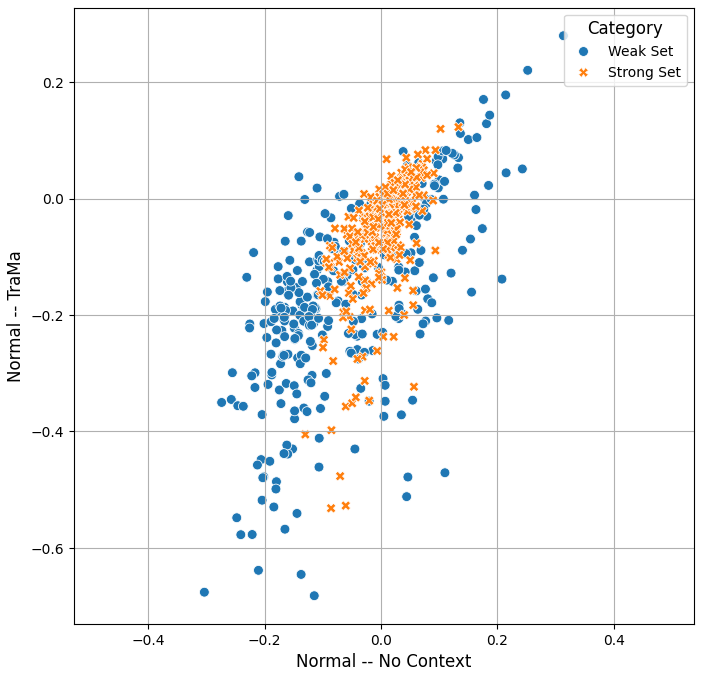
\includegraphics[width=\linewidth]{figures/trama_results.png}
    \caption{
        Changes in RoBERTa model forecast probabilities due to the absence of conversational context (Normal --- No-Context) and the TraMa change of conversational context (Normal --- TraMa).}
    \label{fig:trama-results}
\end{figure}

Using the TraMa test, we can validate our hypothesis that the model, when encountering highly escalatory utterances, may largely overlook the broader conversational context. This can be assessed by measuring the difference in the probability of derailment between the real sample and the ChatGPT-generated TraMa sample, as demonstrated by the two samples in Table~\ref{tab:trama-example}. 

Figure~\ref{fig:trama-results} presents the results of our analysis using the TraMa behavioral test. 
The plot compares the change in RoBERTa model forecast probabilities in the no-context setting and the TraMa setting for the Strong and Weak awry sets.
The findings suggest that while context influences CGA model predictions on CMV, its impact is less when the utterance belongs to the Strong awry set. 
Notably, all 10 RoBERTa models consistently predict such samples as going awry. 
This is evident in Figure~\ref{fig:trama-results}, where the samples from the Strong set are densely clustered around the $(0, 0)$ point. 

Additionally, the points tend to be below the $y=x$ line, suggesting that the TraMa setting resulted in a greater decrease in forecast probabilities compared to the no-context setting. 
To test the statistical significance of these results, a paired t-test was run.
The p-values for the Weak set, Strong set, and combining both sets were all strongly significant ($p < 0.0001$). 
This suggests that the models do in fact utilize conversational context to some degree when making forecasts. 
Combined, these results indicate that SOTA models do utilize conversational context when making forecasts, but the impact of context is less pronounced when the utterance is highly escalatory.

{\color{blue}
\xhdr{Baseline Comparison}
To provide a baseline for comparison, we also conduct the TraMa test on a nonsense context.
\footnote{As suggested by Prof. DNM in an in-class discussion}
Rather than using ChatGPT to generate the preceding context, we use the following fixed context as the preceding utterance: 

{\ttfamily
\begin{align*}
& \text{Thank you so much. I really}\\
& \text{appreciate your help.}\\
\end{align*}
}

We measure the change in RoBERTa model forecast probabilities between the normal setting and the nonsense context sample.
We then compare this change with the change observed in the TraMa setting. 
A paired t-test was run to test the statistical significance of the results.
We find that the decrease in forecast probabilities due to TraMa context is significantly greater than the decrease due to the nonsense context ($p < 0.0001$).
This suggests that the TraMa context is more effective at altering the forecast probabilities than a nonsense context, further supporting our finding that the model utilizes conversational context when making utterance-level forecasts.
}

\xhdr{Human Annotation Task}
%
To understand whether or not humans use the conversational context to make forecasts, 
we conducted a human annotation task. 
%
In this task, the participants were shown 20 single utterances from different 
conversations, 10 of which are awry and the other 10 of which are calm. 
%
Then, they are asked to predict whether each single utterance is awry 
or not, without having access to the prior context.
%
This task was performed by all of our group members, as well as two other students 
in the class, totaling 5 participants. 
%
In this setting, we find that the average accuracy of all the participants is 80\%. 
%
Thus, our results indicate that humans can also achieve relatively impressive 
performance on this task without using the conversational context.

\section{Course Project Specifics}

\subsection{Project Changes over the Semester}

Over the course of the semester, our project has remained largely consistent.
Our overall research goal of understanding how SOTA models use conversational context in making predictions has not changed.
However, we were able to refine our research questions as we progressed.
In particular, whether these models need to use context, and whether these models actually use context, are distinct questions that we distilled from our overarching research goal.

\subsection{Individual Contributions}
Son was primarily responsible for running the model evaluations. 
Austin and Vivian were primarily responsible for trying ChatGPT prompts to use, as well as designing and running the human annotations.
All three team members contributed equally to the presentations and writing of the paper.

\section{Future Work}

\section{Conclusion}


\section*{Acknowledgments}

You can use the command \verb|\citet| (cite in text) to get ``author (year)'' citations, like this citation to a paper by \citet{Gusfield:97}.
You can use the command \verb|\citep| (cite in parentheses) to get ``(author, year)'' citations \citep{Gusfield:97}.
You can use the command \verb|\citealp| (alternative cite without parentheses) to get ``author, year'' citations, which is useful for using citations within parentheses (e.g. \citealp{Gusfield:97}).

A possessive citation can be made with the command \verb|\citeposs|.
This is not a standard natbib command, so it is generally not compatible
with other style files.

This document has been adapted
by Steven Bethard, Ryan Cotterell and Rui Yan
from the instructions for earlier ACL and NAACL proceedings, including those for
ACL 2019 by Douwe Kiela and Ivan Vuli\'{c},
NAACL 2019 by Stephanie Lukin and Alla Roskovskaya,
ACL 2018 by Shay Cohen, Kevin Gimpel, and Wei Lu,
NAACL 2018 by Margaret Mitchell and Stephanie Lukin,
Bib\TeX{} suggestions for (NA)ACL 2017/2018 from Jason Eisner,
ACL 2017 by Dan Gildea and Min-Yen Kan,
NAACL 2017 by Margaret Mitchell,
ACL 2012 by Maggie Li and Michael White,
ACL 2010 by Jing-Shin Chang and Philipp Koehn,
ACL 2008 by Johanna D. Moore, Simone Teufel, James Allan, and Sadaoki Furui,
ACL 2005 by Hwee Tou Ng and Kemal Oflazer,
ACL 2002 by Eugene Charniak and Dekang Lin,
and earlier ACL and EACL formats written by several people, including
John Chen, Henry S. Thompson and Donald Walker.
Additional elements were taken from the formatting instructions of the \emph{International Joint Conference on Artificial Intelligence} and the \emph{Conference on Computer Vision and Pattern Recognition}.

% Bibliography entries for the entire Anthology, followed by custom entries
%\bibliography{anthology,custom}
% Custom bibliography entries only
\bibliography{custom}

\appendix

\end{document}
